\heading{数据结构与算法B-22春-期末}
\textbf{一、选择题（30 分，每小题 2 分）}

\begin{question}
双向链表中的每个结点有两个引用域 \texttt{prev} 和 \texttt{next}，分别引用当前结点的前驱与后继。设 \texttt{p} 引用链表中的一个结点，\texttt{q} 引用一待插入结点，现要求在 \texttt{p} 前插入 \texttt{q}，正确的插入操作为（\quad）。
\begin{choiceoptions}[1]
  \item \texttt{p.prev=q; q.next=p; p.prev.next=q; q.prev=p.prev;}
  \item \texttt{q.prev=p.prev; p.prev.next=q; q.next=p; p.prev=q.next;}
  \item \texttt{q.next=p; p.next=q; p.prev.next=q; q.next=p;}
  \item \texttt{p.prev.next=q; q.next=p; q.prev=p.prev; p.prev=q;}
\end{choiceoptions}
\begin{solution}
选 D。该操作先令原前驱指向 \texttt{q}，再令 \texttt{q} 指向 \texttt{p}，最后修正 \texttt{q.prev} 与 \texttt{p.prev}。
\end{solution}
\end{question}

\begin{question}
给定一个 $N$ 个相异元素构成的有序数列，设计递归算法实现二分查找。考察递归过程中栈的使用情况，该递归调用栈的最小容量应为（\quad）。
\begin{choiceoptions}[2]
  \item $N$
  \item $N/2$
  \item $\lfloor \log_2 N\rfloor$
  \item $\lceil \log_2 (N+1)\rceil$
\end{choiceoptions}
\begin{solution}
选 D。递归二分查找的最大递归深度等于判定树的高度，量级为 $\lceil\log_2(N+1)\rceil$。
\end{solution}
\end{question}

\begin{question}
数据结构有三个基本要素：逻辑结构、存储结构以及基于结构定义的行为（运算）。下列概念中，（\quad）属于存储结构。
\begin{choiceoptions}[2]
  \item 线性表
  \item 链表
  \item 字符串
  \item 二叉树
\end{choiceoptions}
\begin{solution}
选 B。链表是线性表的一种链式存储结构；其余选项通常指逻辑结构。
\end{solution}
\end{question}

\begin{question}
采用数组 $Q[0..m-1]$ 实现循环队列，变量 \texttt{rear} 表示队尾元素的实际位置，添加结点时按 $\texttt{rear}=(\texttt{rear}+1)\%m$ 移动，变量 \texttt{length} 表示当前队列中的元素个数，则队首元素的实际位置是（\quad）。
\begin{choiceoptions}[1]
  \item $\texttt{rear}-\texttt{length}$
  \item $(1+\texttt{rear}+m-\texttt{length})\%m$
  \item $(\texttt{rear}-\texttt{length}+m)\%m$
  \item $m-\texttt{length}$
\end{choiceoptions}
\begin{solution}
选 B。队尾为最后一个元素，因此队首下标为 $\texttt{rear}-\texttt{length}+1$，取模后即选项 B。
\end{solution}
\end{question}

\begin{question}
给定一棵二叉树，若前序遍历序列与中序遍历序列相同，则该二叉树是（\quad）。
\begin{choiceoptions}[2]
  \item 根结点无左子树的二叉树
  \item 根结点无右子树的二叉树
  \item 只有根结点的二叉树或非叶子结点只有左子树的二叉树
  \item 只有根结点的二叉树或非叶子结点只有右子树的二叉树
\end{choiceoptions}
\begin{solution}
选 D。若每个非叶结点都无左子树，则前序和中序都按“根、右子树”访问；反之若某结点有左子树，则中序会先访问其左子树，与前序不同。
\end{solution}
\end{question}

\begin{question}
用 Huffman 算法构造最优二叉编码树，待编码字符权值为 $\{3,4,5,6,8,9,11,12\}$，该树的带权外部路径长度为（\quad）。
\begin{choiceoptions}[2]
  \item $58$
  \item $169$
  \item $72$
  \item $182$
\end{choiceoptions}
\begin{solution}
选 B。依次合并 $3,4$；$5,6$；$7,8$；$9,11$；$11,12$；$15,20$；$23,35$，合并权值和为 $7+11+15+20+23+35+58=169$。
\end{solution}
\end{question}

\begin{question}
若需要对存储开销约 $1\mathrm{GB}$ 的数据排序，而当前可用 RAM 只有 $100\mathrm{MB}$，最适合的排序算法是（\quad）。
\begin{choiceoptions}[2]
  \item 堆排序
  \item 归并排序
  \item 快速排序
  \item 插入排序
\end{choiceoptions}
\begin{solution}
选 B。外部排序常采用多路归并思想，适合数据量显著大于内存容量的情形。
\end{solution}
\end{question}

\begin{question}
一个无向图 $G$ 含有 $18$ 条边，其中度数为 $4$ 的顶点有 $3$ 个，度数为 $3$ 的顶点有 $4$ 个，其他顶点的度数均小于 $3$，则 $G$ 的顶点数至少为（\quad）。
\begin{choiceoptions}[1]
  \item $10$
  \item $11$
  \item $13$
  \item $15$
\end{choiceoptions}
\begin{solution}
选 C。总度数为 $2|E|=36$。已知顶点贡献度数 $3\cdot4+4\cdot3=24$，还差 $12$；其余顶点度数均至多为 $2$，至少还需 $6$ 个顶点，所以总顶点数至少为 $3+4+6=13$。
\end{solution}
\end{question}

\begin{question}
无向图 $G$ 从 $V_0$ 出发作深度优先遍历，访问的树边集合为
\[
\{(V_0,V_1),(V_0,V_4),(V_1,V_2),(V_1,V_3),(V_4,V_5),(V_5,V_6)\}.
\]
则下列哪条边不可能出现在 $G$ 中？（\quad）
\begin{choiceoptions}[2]
  \item $(V_0,V_2)$
  \item $(V_4,V_6)$
  \item $(V_4,V_3)$
  \item $(V_0,V_6)$
\end{choiceoptions}
\begin{solution}
选 C。无向图 DFS 中非树边只能连接祖先与后代。$(V_4,V_3)$ 位于 DFS 树的两个不同分支之间，不可能作为非树边出现。
\end{solution}
\end{question}

\begin{question}
已知有向图 $G$ 的邻接边表如下图所示，
\begin{center}
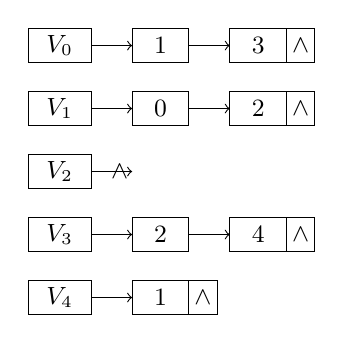
\begin{tikzpicture}[x=8mm,y=8mm,every node/.style={font=\small,inner sep=1pt}]
% header vertex boxes
\foreach \i/\v in {0/$V_0$,1/$V_1$,2/$V_2$,3/$V_3$,4/$V_4$}{
  \draw (0,-\i) rectangle (1,-\i-0.55);
  \node at (0.5,-\i-0.275) {\v};
  \draw[->] (1,-\i-0.275) -- (1.65,-\i-0.275);
}
% V0: 1 -> 3 -> null
\draw (1.65,0) rectangle (2.55,-0.55); \node at (2.1,-0.275) {1};
\draw[->] (2.55,-0.275) -- (3.2,-0.275);
\draw (3.2,0) rectangle (4.1,-0.55); \node at (3.65,-0.275) {3};
\draw (4.1,0) rectangle (4.55,-0.55); \node at (4.325,-0.275) {$\wedge$};
% V1: 0 -> 2 -> null
\draw (1.65,-1) rectangle (2.55,-1.55); \node at (2.1,-1.275) {0};
\draw[->] (2.55,-1.275) -- (3.2,-1.275);
\draw (3.2,-1) rectangle (4.1,-1.55); \node at (3.65,-1.275) {2};
\draw (4.1,-1) rectangle (4.55,-1.55); \node at (4.325,-1.275) {$\wedge$};
% V2 null
\node at (1.45,-2.275) {$\wedge$};
% V3: 2 -> 4 -> null
\draw (1.65,-3) rectangle (2.55,-3.55); \node at (2.1,-3.275) {2};
\draw[->] (2.55,-3.275) -- (3.2,-3.275);
\draw (3.2,-3) rectangle (4.1,-3.55); \node at (3.65,-3.275) {4};
\draw (4.1,-3) rectangle (4.55,-3.55); \node at (4.325,-3.275) {$\wedge$};
% V4: 1 -> null
\draw (1.65,-4) rectangle (2.55,-4.55); \node at (2.1,-4.275) {1};
\draw (2.55,-4) rectangle (3.0,-4.55); \node at (2.775,-4.275) {$\wedge$};
\end{tikzpicture}
\end{center}
从 $V_0$ 出发进行深度优先周游，得到的 DFS 结点序列为（\quad）。
\begin{choiceoptions}[2]
  \item $V_0,V_1,V_4,V_3,V_2$
  \item $V_0,V_1,V_2,V_3,V_4$
  \item $V_0,V_1,V_3,V_2,V_4$
  \item $V_0,V_2,V_1,V_3,V_4$
\end{choiceoptions}
\begin{solution}
选 B。按邻接表顺序访问：$V_0\to V_1\to V_2$，回溯后由 $V_0\to V_3\to V_4$，故序列为 $V_0,V_1,V_2,V_3,V_4$。
\end{solution}
\end{question}

\begin{question}
若按排序的稳定性对排序算法分类，下列算法中不稳定的是（\quad）。
\begin{choiceoptions}[2]
  \item 冒泡排序
  \item 归并排序
  \item 直接插入排序
  \item 希尔排序
\end{choiceoptions}
\begin{solution}
选 D。希尔排序可能使相同关键码的元素跨间隔交换，通常不稳定。
\end{solution}
\end{question}

\begin{question}
下列哪组排序算法的最好情况下时间复杂度的大 $O$ 表示相同？（\quad）
\begin{choiceoptions}[2]
  \item 快速排序和堆排序
  \item 归并排序和插入排序
  \item 快速排序和选择排序
  \item 堆排序和冒泡排序
\end{choiceoptions}
\begin{solution}
选 A。快速排序最好为 $O(n\log n)$，堆排序各情形均为 $O(n\log n)$。
\end{solution}
\end{question}

\begin{question}
设结点 $X$ 和 $Y$ 是二叉树中任意两个结点。若在该树的先根周游序列中 $X$ 出现在 $Y$ 之前，而在其后根周游序列中 $X$ 出现在 $Y$ 之后，则 $X$ 与 $Y$ 的关系是（\quad）。
\begin{choiceoptions}[1]
  \item $X$ 是 $Y$ 的左兄弟
  \item $X$ 是 $Y$ 的右兄弟
  \item $X$ 是 $Y$ 的祖先
  \item $X$ 是 $Y$ 的后裔
\end{choiceoptions}
\begin{solution}
选 C。祖先结点在前序中先于后代访问，在后序中后于后代访问。
\end{solution}
\end{question}

\begin{question}
森林 $F$ 中每个结点的子结点数均不超过 $2$。若森林 $F$ 中叶子结点总数为 $L$，度数为 $2$ 的结点总数为 $N$，则森林 $F$ 中树的个数为（\quad）。
\begin{choiceoptions}[1]
  \item $L-N-1$
  \item 无法确定
  \item $L-N$
  \item $N-L$
\end{choiceoptions}
\begin{solution}
选 C。设度为 $1$ 的结点数为 $N_1$，树的棵数为 $t$。边数为 $L+N_1+N-t$，也等于 $N_1+2N$，所以 $t=L-N$。
\end{solution}
\end{question}

\begin{question}
回溯法是一类广泛使用的算法，下列叙述中不正确的是（\quad）。
\begin{choiceoptions}[2]
  \item 回溯法可以系统地搜索一个问题的所有解或者任意解
  \item 回溯法是一种既具系统性又具跳跃性的搜索算法
  \item 回溯算法需要借助队列数据结构来保存从根结点到当前扩展结点的路径
  \item 回溯法在生成解空间的任一结点时，先判断当前结点是否可能包含问题的有效解；若肯定不包含，则跳过对该结点为根的子树的搜索，逐层向祖先结点回溯
\end{choiceoptions}
\begin{solution}
选 C。回溯通常借助递归栈或显式栈保存路径，而不是队列。
\end{solution}
\end{question}


\textbf{二、判断题（10 分，每小题 1 分；对填 Y，错填 N）}

\begin{question}
对任意一个连通的、无环的无向图，从图中移除任何一条边得到的图均不连通。（\quad）
\begin{solution}
答案：Y。连通且无环的无向图就是树。树中任意一条边都是桥，删除任何一条边都会把原来的树分成两个连通分量，因此所得图不再连通。
\end{solution}
\end{question}

\begin{question}
给定二叉树，前序周游序列为 \texttt{HGEDBFCA}、中序周游序列为 \texttt{EGBDHFAC} 时，其后序周游序列必为 \texttt{EBDGACFH}。（\quad）
\begin{solution}
答案：Y。前序第一个结点 $H$ 是根；中序序列以 $H$ 分成左子树 \texttt{EGBD} 和右子树 \texttt{FAC}。递归划分左子树可得后序 \texttt{EBDG}，右子树可得后序 \texttt{ACF}，最后访问根 $H$，合并为 \texttt{EBDGACFH}。
\end{solution}
\end{question}

\begin{question}
对结点值在 $1$ 到 $1000$ 之间的二叉搜索树查找 $363$，以下三个序列皆可能为查找路径：
\[
\begin{array}{@{}l@{}}
\text{A}.\ 2,252,401,398,330,344,397,363;\\
\text{B}.\ 925,202,911,240,912,245,363;\\
\text{C}.\ 935,278,347,621,299,392,358,363.
\end{array}
\]
（\quad）
\begin{solution}
答案：N。二叉搜索树查找路径必须满足逐步收缩的区间约束：若当前结点大于 $363$，下一步只能进入左子树，上界随之变小；若当前结点小于 $363$，下一步只能进入右子树，下界随之变大。序列 A 满足区间约束；序列 B 中，访问 $911$ 后若目标 $363$ 位于其左子树，则后续结点必须小于 $911$，但下一步出现 $912$，矛盾；序列 C 中，访问 $347$ 后目标位于其右子树，后续结点必须大于 $347$，但之后出现 $299$，矛盾。因此不能说“三个序列皆可能”。
\end{solution}
\end{question}

\begin{question}
构建一个含 $N$ 个结点的（二叉）最小值堆，建堆时间复杂度的大 $O$ 表示为 $O(N\log N)$。（\quad）
\begin{solution}
答案：N。若采用自底向上的筛选建堆方法（常称 Floyd 建堆），从最后一个非叶子结点开始下滤调整，整体时间复杂度为 $O(N)$。$O(N\log N)$ 是逐个插入建堆的一种上界，不是通常“建堆”算法的紧确复杂度。
\end{solution}
\end{question}

\begin{question}
队列是动态集合，其定义的出队列操作所移除的元素总是在集合中存在时间最长的元素。（\quad）
\begin{solution}
答案：Y。队列遵循先进先出（FIFO）原则，最早进入队列且尚未出队的元素会最先被删除。因此出队操作删除的是当前队列中等待时间最长的元素。
\end{solution}
\end{question}

\begin{question}
任一有向图的拓扑序列既可以通过深度优先搜索求解，也可以通过宽度优先搜索求解。（\quad）
\begin{solution}
答案：Y。拓扑排序可用 DFS：按完成时间逆序输出；也可用 BFS 思想的 Kahn 算法：反复选取入度为 $0$ 的顶点并删除其出边。两类方法都能求有向无环图的拓扑序列。
\end{solution}
\end{question}

\begin{question}
对任一连通无向图 $G$，其中 $E$ 是权值最小的边，那么 $E$ 必然属于任何一个最小生成树。（\quad）
\begin{solution}
答案：N。若权值最小的边不唯一，某一条最小权边未必出现在所有最小生成树中。例如一个三角形三条边权相同，任取两条即可构成最小生成树，第三条最小权边就不在该生成树中。若额外说明“唯一最小边”，结论才成立。
\end{solution}
\end{question}

\begin{question}
对一个包含负权值边的图，Dijkstra 算法总能够给出最短路径问题的正确答案。（\quad）
\begin{solution}
答案：N。Dijkstra 算法依赖“当前最小暂定距离一旦选定就不会再被改小”的性质，该性质要求边权非负。存在负权边时，已经确定的顶点距离可能通过之后的负边再次变小，因此算法不保证正确。
\end{solution}
\end{question}

\begin{question}
分治算法通常将原问题分解为几个规模较小但类似于原问题的子问题，递归求解这些子问题，然后再合并子问题的解来建立原问题的解。（\quad）
\begin{solution}
答案：Y。这正是分治法的基本框架：分解、递归求解、合并。归并排序就是典型例子，它先把序列分成较小子序列，分别排序，再把有序子序列合并。
\end{solution}
\end{question}

\begin{question}
考察某个具体问题是否适合应用动态规划算法，必须判定它是否具有最优子结构性质。（\quad）
\begin{solution}
答案：Y。动态规划要求原问题的最优解能够由子问题的最优解组合而来，这称为最优子结构。若不具备该性质，就不能直接通过保存并组合子问题最优解来保证原问题最优。
\end{solution}
\end{question}

\textbf{三、填空题（20 分，每题 2 分）}

\begin{question}
目标串长为 $n$、模式串长为 $m$，朴素模式匹配算法中字符最多比较次数为 \blank。
\begin{solution}
答案：$(n-m+1)m$，数量级为 $O(nm)$。朴素匹配最多要尝试 $n-m+1$ 个起始位置；在最坏情况下，每个起始位置都比较到模式串最后一个字符才失败或成功，因此最多比较 $(n-m+1)m$ 次。
\end{solution}
\end{question}

\begin{question}
一棵含 $n$ 个结点的树中，只有度为 $k$ 的分支结点和度为 $0$ 的终端结点，则终端结点数为 \blank。
\begin{solution}
答案：$\dfrac{(k-1)n+1}{k}$。设度为 $k$ 的分支结点数为 $x$，终端结点数为 $n_0$，则 $x+n_0=n$。树的边数为 $n-1$，又等于所有结点度数之和 $kx$，所以 $kx=n-1$，$x=(n-1)/k$，从而 $n_0=n-(n-1)/k=\dfrac{(k-1)n+1}{k}$。
\end{solution}
\end{question}

\begin{question}
对关键码序列 $\{46,70,56,38,40,80\}$ 作快速排序，以第一个记录为基准的一次划分结果为 \blank。
\begin{solution}
答案：$40,38,46,56,70,80$。以 $46$ 为基准，划分后所有小于 $46$ 的关键码应在其左侧，所有大于 $46$ 的关键码应在其右侧。按常见左右交替扫描的划分过程，可得到 $40,38,46,56,70,80$。
\end{solution}
\end{question}

\begin{question}
长度为 $3$ 的顺序表中，查找第一个、第二个、第三个元素的概率分别为 $1/2,1/4,1/8$。若剩余概率理解为查找失败且失败需比较 $3$ 次，则平均比较次数为 \blank。
\begin{solution}
答案：$\dfrac{7}{4}$。查找成功时，三个位置的比较次数分别为 $1,2,3$；成功概率总和为 $1/2+1/4+1/8=7/8$，剩余失败概率为 $1/8$，失败需比较 $3$ 次。因此平均比较次数为 $1\cdot\frac12+2\cdot\frac14+3\cdot\frac18+3\cdot\frac18=\frac74$。
\end{solution}
\end{question}

\begin{question}
关键码为 $\{19,14,23,1,68,20,84,27,55,11,10,79\}$，用链地址法和 $H(\mathrm{key})=\mathrm{key}\bmod 13$ 构造散列表，则地址为 $1$ 的链中有 \blank 个记录。
\begin{solution}
答案：$4$。逐个计算模 $13$ 的余数：$14\bmod13=1$，$1\bmod13=1$，$27\bmod13=1$，$79\bmod13=1$。其余关键码的余数不是 $1$，所以地址 $1$ 的链中共有 $4$ 个记录。
\end{solution}
\end{question}

\begin{question}
删除长度为 $n$ 的顺序表第 $i$ 个数据元素需要移动表中的 \blank 个数据元素。
\begin{solution}
答案：$n-i$。顺序表删除第 $i$ 个元素后，原来第 $i+1$ 到第 $n$ 个元素都要依次前移一位，共有 $n-i$ 个元素需要移动。
\end{solution}
\end{question}

\begin{question}
小根堆为 $[8,15,10,21,34,16,12]$，删除关键字 $8$ 并重新建堆时，关键字比较次数为 \blank。
\begin{solution}
答案：$3$。删除堆顶 $8$ 后，用最后一个元素 $12$ 补到根，得到 $[12,15,10,21,34,16]$。先比较两个孩子 $15$ 和 $10$，再比较 $12$ 与较小孩子 $10$，交换后再比较 $12$ 与其孩子 $16$，共 $3$ 次关键字比较。
\end{solution}
\end{question}

\begin{question}
在广度优先遍历、拓扑排序、求最短路径三种算法中，可判断有向图是否有环的是 \blank。
\begin{solution}
答案：拓扑排序。有向图存在拓扑序列当且仅当它是有向无环图。若拓扑排序过程中仍有顶点未输出但不存在入度为 $0$ 的顶点，则说明图中存在有向环。
\end{solution}
\end{question}

\begin{question}
$n\;(n\ge2)$ 个顶点的有向强连通图最少有 \blank 条边。
\begin{solution}
答案：$n$。要使每个顶点都能到达其他顶点，最少可以构成一个包含全部 $n$ 个顶点的有向环，此时有 $n$ 条有向边，并且任意两点互相可达。少于 $n$ 条边不可能让所有顶点都处在同一个强连通结构中。
\end{solution}
\end{question}

\begin{question}
栈 $S_1$ 中操作数自栈底到栈顶为 $5,8,3,2$，栈 $S_2$ 中运算符自栈底到栈顶为 $*, -, /$，按题给函数调用三次后，若按整数除法计算，$S_1$ 栈顶为 \blank。
\begin{solution}
答案：$35$。第一次弹出运算符 $/$，用栈顶两个操作数计算 $3/2=1$（整数除法），$S_1$ 变为 $5,8,1$；第二次弹出 $-$，计算 $8-1=7$，$S_1$ 变为 $5,7$；第三次弹出 $*$，计算 $5\times7=35$，故最终栈顶为 $35$。
\end{solution}
\end{question}

\textbf{四、简答题（3 题，共 20 分）}
\begin{question}[Dijkstra 算法]
试用 Dijkstra 算法求题图中顶点 $1$ 到其余各顶点的最短路径，写出算法执行过程中各步状态。
\begin{center}
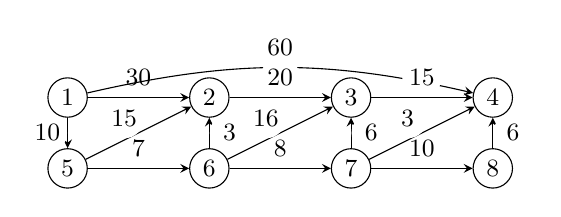
\begin{tikzpicture}[x=9mm,y=9mm,every node/.style={draw,circle,font=\small,minimum size=5mm,inner sep=0pt},>=stealth]
\node (v1) at (0,1) {1}; \node (v2) at (2,1) {2}; \node (v3) at (4,1) {3}; \node (v4) at (6,1) {4};
\node (v5) at (0,0) {5}; \node (v6) at (2,0) {6}; \node (v7) at (4,0) {7}; \node (v8) at (6,0) {8};
\draw[->] (v1) -- node[above,draw=none,fill=white] {30} (v2);
\draw[->] (v1) -- node[left,draw=none,fill=white] {10} (v5);
\draw[->] (v1) to[bend left=13] node[above,draw=none,fill=white] {60} (v4);
\draw[->] (v5) -- node[above,draw=none,fill=white] {7} (v6);
\draw[->] (v5) -- node[above left,draw=none,fill=white] {15} (v2);
\draw[->] (v6) -- node[right,draw=none,fill=white] {3} (v2);
\draw[->] (v2) -- node[above,draw=none,fill=white] {20} (v3);
\draw[->] (v6) -- node[above,draw=none,fill=white] {8} (v7);
\draw[->] (v6) -- node[above left,draw=none,fill=white] {16} (v3);
\draw[->] (v7) -- node[right,draw=none,fill=white] {6} (v3);
\draw[->] (v7) -- node[above,draw=none,fill=white] {10} (v8);
\draw[->] (v7) -- node[above left,draw=none,fill=white] {3} (v4);
\draw[->] (v3) -- node[above,draw=none,fill=white] {15} (v4);
\draw[->] (v8) -- node[right,draw=none,fill=white] {6} (v4);
\end{tikzpicture}
\end{center}
\begin{center}
\footnotesize
\begin{tabular}{c c c c c c c c c c}
\toprule
所选顶点 & $U$（已确定最短路径的顶点集合） & $T$（未确定最短路径的顶点集合） & $d_2$ & $d_3$ & $d_4$ & $d_5$ & $d_6$ & $d_7$ & $d_8$ \\
\midrule
初始 & $\{1\}$ & $\{2,3,4,5,6,7,8\}$ & 30 & $\infty$ & 60 & 10 & $\infty$ & $\infty$ & $\infty$ \\
 & & & & & & & & & \\
 & & & & & & & & & \\
 & & & & & & & & & \\
 & & & & & & & & & \\
 & & & & & & & & & \\
 & & & & & & & & & \\
 & & & & & & & & & \\
\bottomrule
\end{tabular}
\end{center}

\begin{solution}
按题图边权，从顶点 $1$ 出发。用 $d(i)$ 表示当前从 $1$ 到 $i$ 的最短估计距离，$\infty$ 表示暂不可达。执行过程如下：
\begin{center}
\begin{tabular}{c|c|ccccccc}
\toprule
步骤 & 新确定顶点 & $d(2)$ & $d(3)$ & $d(4)$ & $d(5)$ & $d(6)$ & $d(7)$ & $d(8)$ \\
\midrule
0 & 1 & 30 & $\infty$ & 60 & 10 & $\infty$ & $\infty$ & $\infty$ \\
1 & 5 & 25 & $\infty$ & 60 & 10 & 17 & $\infty$ & $\infty$ \\
2 & 6 & 20 & 33 & 60 & 10 & 17 & 25 & $\infty$ \\
3 & 2 & 20 & 33 & 60 & 10 & 17 & 25 & $\infty$ \\
4 & 7 & 20 & 31 & 28 & 10 & 17 & 25 & 35 \\
5 & 4 & 20 & 31 & 28 & 10 & 17 & 25 & 35 \\
6 & 3 & 20 & 31 & 28 & 10 & 17 & 25 & 35 \\
7 & 8 & 20 & 31 & 28 & 10 & 17 & 25 & 35 \\
\bottomrule
\end{tabular}
\end{center}
因此选点次序为 $1,5,6,2,7,4,3,8$，最短距离为
\[
(d_2,d_3,d_4,d_5,d_6,d_7,d_8)=(20,31,28,10,17,25,35).
\]
一组对应路径为：$1\to5\to6\to2$，$1\to5\to6\to7\to3$，$1\to5\to6\to7\to4$，$1\to5$，$1\to5\to6$，$1\to5\to6\to7$，$1\to5\to6\to7\to8$。
\end{solution}
\end{question}

\begin{question}[二叉搜索树]
给定关键码集合 $\{18,73,5,10,68,99,27\}$。
\begin{enumerate}
  \item 画出按记录顺序构造形成的二叉排序（搜索）树；
  \item 画出删除关键码 $73$ 后的二叉排序树；
  \item 画出对集合 $C$（未删除 $73$ 前）查询效率最高的最优二叉排序树，其中每个关键码被查询概率相等。
\end{enumerate}
\begin{solution}
顺序插入得到：根为 $18$；左子树为 $5$，且 $5$ 的右孩子为 $10$；右子树根为 $73$，$73$ 的左孩子为 $68$、右孩子为 $99$，$68$ 的左孩子为 $27$。
\begin{center}
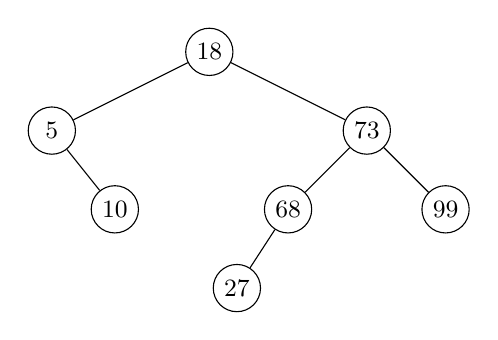
\begin{tikzpicture}[x=1cm,y=1cm,every node/.style={draw,circle,font=\small,minimum size=6mm,inner sep=0pt}]
\node (a18) at (0,0) {18};
\node (a5) at (-2,-1) {5};
\node (a73) at (2,-1) {73};
\node (a10) at (-1.2,-2) {10};
\node (a68) at (1,-2) {68};
\node (a99) at (3,-2) {99};
\node (a27) at (0.35,-3) {27};
\foreach \u/\v in {a18/a5,a18/a73,a5/a10,a73/a68,a73/a99,a68/a27}
  \draw (\u)--(\v);
\end{tikzpicture}
\end{center}

删除 $73$ 时，可用其左子树最大结点 $68$ 替代，得到右子树根 $68$，其左孩子为 $27$、右孩子为 $99$。
\begin{center}
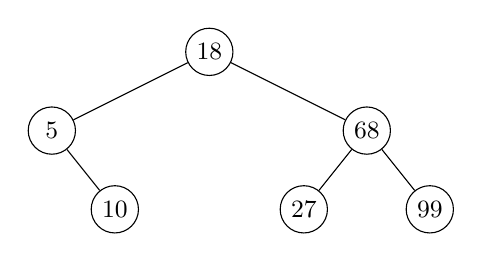
\begin{tikzpicture}[x=1cm,y=1cm,every node/.style={draw,circle,font=\small,minimum size=6mm,inner sep=0pt}]
\node (b18) at (0,0) {18};
\node (b5) at (-2,-1) {5};
\node (b68) at (2,-1) {68};
\node (b10) at (-1.2,-2) {10};
\node (b27) at (1.2,-2) {27};
\node (b99) at (2.8,-2) {99};
\foreach \u/\v in {b18/b5,b18/b68,b5/b10,b68/b27,b68/b99}
  \draw (\u)--(\v);
\end{tikzpicture}
\end{center}

若在原集合 $\{5,10,18,27,68,73,99\}$ 上等概率查找，最优二叉排序树可取中位数 $27$ 为根，左子树根为 $10$、右子树根为 $73$，叶结点为 $5,18,68,99$。这是高度尽量平衡的二叉搜索树，成功查找平均比较次数最小。
\begin{center}
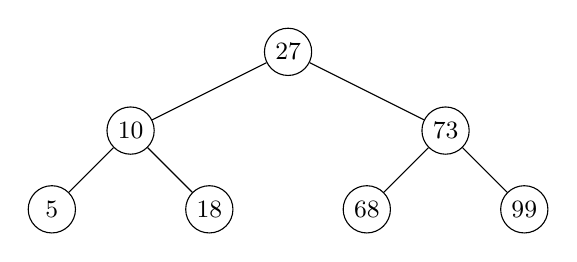
\begin{tikzpicture}[x=1cm,y=1cm,every node/.style={draw,circle,font=\small,minimum size=6mm,inner sep=0pt}]
\node (c27) at (0,0) {27};
\node (c10) at (-2,-1) {10};
\node (c73) at (2,-1) {73};
\node (c5) at (-3,-2) {5};
\node (c18) at (-1,-2) {18};
\node (c68) at (1,-2) {68};
\node (c99) at (3,-2) {99};
\foreach \u/\v in {c27/c10,c27/c73,c10/c5,c10/c18,c73/c68,c73/c99}
  \draw (\u)--(\v);
\end{tikzpicture}
\end{center}
\end{solution}
\end{question}

\begin{question}[奇偶交换排序]
奇偶交换排序如下：第一趟对所有奇数 $i$ 比较 $a_i$ 与 $a_{i+1}$，必要时交换；第二趟对所有偶数 $i$ 比较 $a_i$ 与 $a_{i+1}$，必要时交换；如此交替，直到整个序列有序。对序列 $\{18,73,5,10,68,99,27,10\}$ 写出前 $4$ 趟结果，说明算法是否稳定，并给出正序、逆序输入时的比较次数和交换次数。
\begin{solution}
前 $4$ 趟结果依次为
\[
\begin{aligned}
&18,73,5,10,68,99,10,27,\\
&18,5,73,10,68,10,99,27,\\
&5,18,10,73,10,68,27,99,\\
&5,10,18,10,73,27,68,99.
\end{aligned}
\]
算法只在相邻元素逆序时交换，相等元素不交换，因此是稳定排序。

若初始序列为正序，比较 $n-1$ 次，交换 $0$ 次。若初始序列为逆序，则每个逆序对最终都要通过一次相邻交换消去，交换次数为
\[
\frac{n(n-1)}{2}.
\]
按题给停止条件，最后还需一轮无交换检查，比较次数为
\[
\frac{n(n-1)}{2}+n-1.
\]
\end{solution}
\end{question}

\textbf{五、算法填空（2 题，共 20 分）}

\begin{question}[单链表逆置]
填空完成程序：读入整数序列，用单链表存储，然后将该单链表原地逆置后输出。下面程序使用普通头引用 \texttt{head}，链表结点定义为 \texttt{Node(data)}。

\begin{pycode}
class Node:
    def __init__(self, data):
        self.data = data
        self.next = None


def print_list(head):
    p = head
    while p is not None:
        print(p.data, end=" ")
        p = p.next
    print()


def reverse_list(head):
    if head is not None:
        p = head.next
        head.next = __________                  # (1)
        while p is not None:
            q = p
            p = __________                      # (2)
            q.next = __________                 # (3)
            __________                          # (4)
    return head

n = int(input())
a = list(map(int, input().split()))
head = Node(a[0])
p = head
for i in range(1, n):
    p.next = __________                         # (5)
    p = __________                              # (6)

head = reverse_list(head)
print_list(head)
\end{pycode}
\begin{solution}
填空答案：(1) \texttt{None}；(2) \texttt{p.next}；(3) \texttt{head}；(4) \texttt{head = q}；(5) \texttt{Node(a[i])}；(6) \texttt{p.next}。

逆置时，先把原头结点变成新链表的尾结点，即令 \texttt{head.next = None}。随后依次取出原链表剩余结点 \texttt{p}，用头插法插入到新链表头部。变量 \texttt{q} 暂存当前结点，\texttt{p} 先后移，随后令 \texttt{q.next} 指向当前新表头，再把 \texttt{head} 更新为 \texttt{q}。
\end{solution}
\end{question}


\begin{question}[由扩充二叉树先序序列构造二叉树]
输入一棵二叉树的扩充二叉树先序序列，其中 \texttt{@} 表示空结点。递归构造该二叉树，并输出其中序遍历序列。

例如输入 \texttt{ABD@@G@@CE@@F@@} 时，对应二叉树的中序遍历为 \texttt{DGBAECF}。

\begin{pycode}
class BinaryTreeNode:
    def __init__(self, data):
        self.data = data
        self.left = None
        self.right = None


s = input().strip()
pos = 0


def build_tree():
    global pos
    ch = s[pos]
    pos += 1
    if ch == "@":
        return __________                       # (1)

    root = __________                           # (2)
    root.left = __________                      # (3)
    root.right = __________                     # (4)
    return root


def inorder(root):
    if root is None:
        return
    __________                                  # (5)
    print(root.data, end="")
    __________                                  # (6)


tree = build_tree()
inorder(tree)
\end{pycode}
\begin{solution}
填空答案：(1) \texttt{None}；(2) \texttt{BinaryTreeNode(ch)}；(3) \texttt{build\_tree()}；(4) \texttt{build\_tree()}；(5) \texttt{inorder(root.left)}；(6) \texttt{inorder(root.right)}。

扩充先序序列的读取规则是“根、左子树、右子树”。遇到 \texttt{@} 表示当前子树为空，直接返回 \texttt{None}；否则建立当前根结点，并继续递归构造左、右子树。中序遍历顺序为“左子树、根、右子树”。
\end{solution}
\end{question}

